%%%%%%%%%%%%%%%%%%%%%%%%%%%%%%%%%%%%%%%%%%%%%%%%%%%%%%%%%%%%%%%%%%%%%%%%%%%%%%%%
%2345678901234567890123456789012345678901234567890123456789012345678901234567890
%        1         2         3         4         5         6         7         8

\documentclass[letterpaper, 10 pt, conference]{ieeeconf}  % Comment this line out if you need a4paper
\usepackage{amsmath, xparse}
\usepackage{amstext}
\usepackage{amsfonts}
\usepackage{float}
\usepackage{graphicx}
\usepackage{hyperref}

%\documentclass[a4paper, 10pt, conference]{ieeeconf}      % Use this line for a4 paper

\IEEEoverridecommandlockouts                              % This command is only needed if
                                                          % you want to use the \thanks command

\overrideIEEEmargins                                      % Needed to meet printer requirements.

%In case you encounter the following error:
%Error 1010 The PDF file may be corrupt (unable to open PDF file) OR
%Error 1000 An error occurred while parsing a contents stream. Unable to analyze the PDF file.
%This is a known problem with pdfLaTeX conversion filter. The file cannot be opened with acrobat reader
%Please use one of the alternatives below to circumvent this error by uncommenting one or the other
%\pdfobjcompresslevel=0
%\pdfminorversion=4

% See the \addtolength command later in the file to balance the column lengths
% on the last page of the document

% The following packages can be found on http:\\www.ctan.org
%\usepackage{graphics} % for pdf, bitmapped graphics files
%\usepackage{epsfig} % for postscript graphics files
%\usepackage{mathptmx} % assumes new font selection scheme installed
%\usepackage{times} % assumes new font selection scheme installed
%\usepackage{amsmath} % assumes amsmath package installed
%\usepackage{amssymb}  % assumes amsmath package installed

\title{\LARGE \bf
Midterm Report: \\ 
\Large AlienGLRenderer Cloth Simulation
}



\author{Arrian Chi% <-this % stops a space
\\
\\
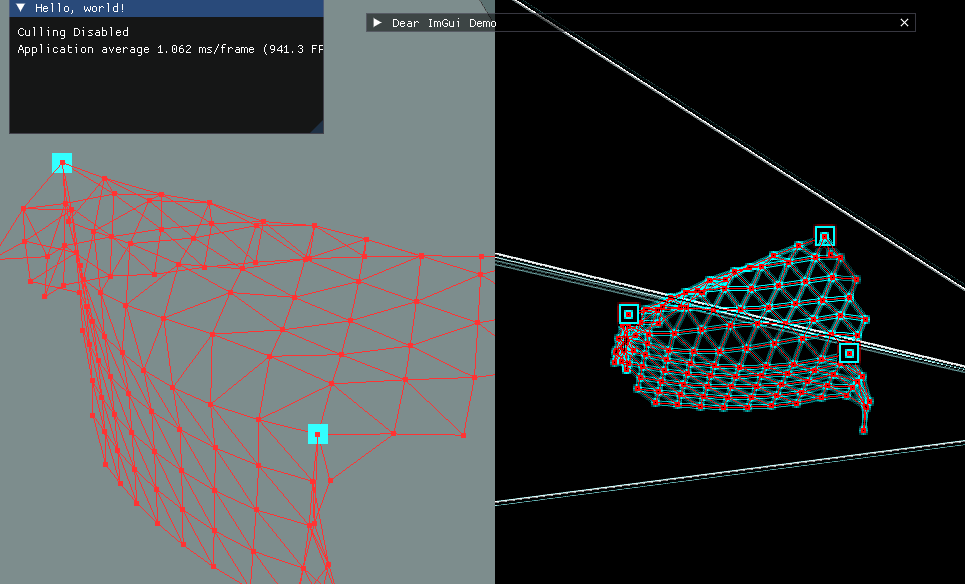
\includegraphics[width=8cm]{cloth1.PNG} \> 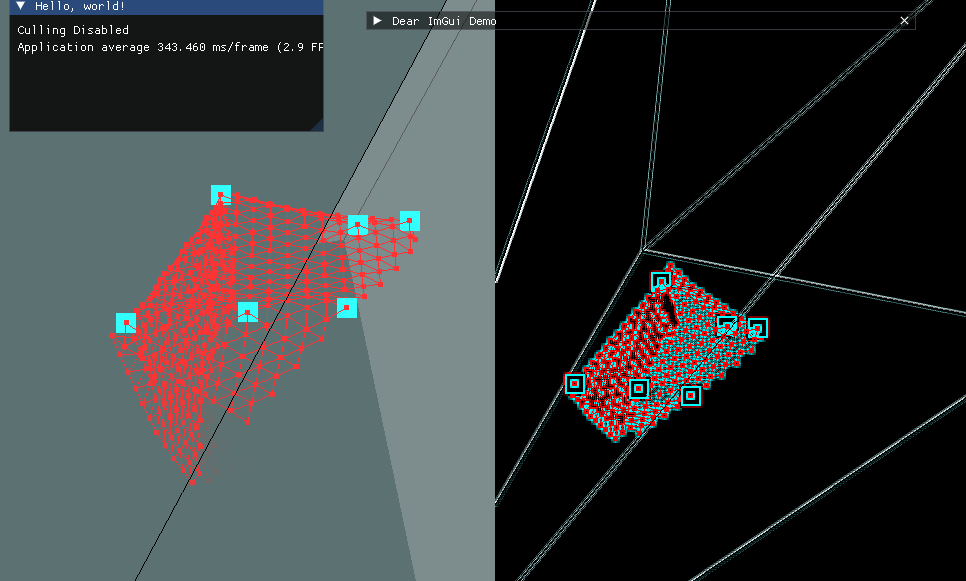
\includegraphics[width=8cm]{cloth2.PNG} 
}




\begin{document}

% \onecolumn


\maketitle
\thispagestyle{empty}
\pagestyle{empty}


%%%%%%%%%%%%%%%%%%%%%%%%%%%%%%%%%%%%%%%%%%%%%%%%%%%%%%%%%%%%%%%%%%%%%%%%%%%%%%%%

\begin{abstract}

        In this midterm report, I present my current progress in the projects, the problems I encountered, and how I managed to mitigate each problem. I will also give an overview of what I plan to complete in the next coming weeks. 

\end{abstract}
\section{Overview}

In my proposal, I mentioned I wanted to create a cloth simulation for my hobby project, AlienGLRenderer. This is essentially a C++ implementation of the DEP/S algorithm \cite{baraff1998large} \cite{Grinspun2003discrete} \cite{Tamstorf2013discrete} we gone over class. However, much emphasis was made on making sure the cloth simulation could run in real-time (online rendering). In the following sections, I will discuss the progress I have made so far, the problems I encountered, and what I plan to do in the next coming weeks. A link to the project may be found here: \url{https://github.com/dinoplane/gl_alien_renderer/tree/main}.

\section{Progress}
Currently, I have a working implementation of the cloth simulation in C++. I will discuss the key components of the simulation below:

\subsection{Cloth Mesh Creation and Parameterization}
The mesh of the cloth is represented as a equilateral triangluar grid of particles connected by edges / hinges. For now, I rendered them points connected by lines, highlighting the points that are fixed in the simulation. Other highlights present in the simulation are used for debug purposes only. The derivation of the points are all procedural and dependent on a user supplied number of edges of the cloth and the edge length. In addition, the user also specifies the young's modulus, the thickness, the gravitational pull, and the timestep of the simulation.

\subsection{Cloth Simulation}
The simulation is based on the DEP/S algorithm we went over in class. The simulation is implicit and is solved using the Newton-Raphson method. The forces acting on the cloth are the internal forces (stretching, bending, and shearing), the external forces (gravity), and the damping forces. The internal forces are calculated using the DEP algorithm, which is a generalization of the StVK model. The external forces are calculated using the gravitational pull and the damping forces are calculated using the velocity of the particles. The forces are calculated in the compute shader and the positions are updated in the update shader. The positions are updated using the implicit Euler method. The simulation is run until the accumulated error in the free forces is less than a certain tolerance.

\begin{figure}[!ht]
        \centering
        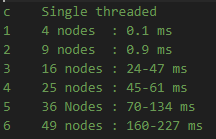
\includegraphics[width=0.25\textwidth,keepaspectratio]{timing_debug.PNG}
        \caption{Average fram times }
        \label{"fig:timing_debug"}
\end{figure}

\begin{figure}[!ht]
        \centering
        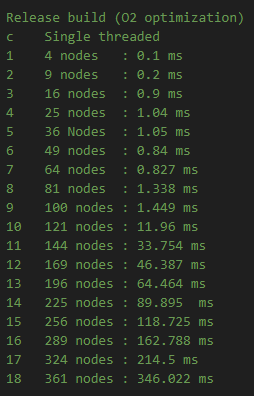
\includegraphics[width=0.25\textwidth,keepaspectratio]{timing_release.PNG}
        \caption{Chaos.}
        \label{"fig:timing_release"}
\end{figure}


\subsection{Current Performance}
The current implementation of the cloth simulation is technically realtime. Figures \ref{"fig:timing_debug"} and \ref{"fig:timing_release"} display the average frame times of the simulation. As you can see, not only is it true that the compute time increases as the number of vertices increases, but also the rate of the compute time is doubling for every square of n. This is definitely not linear growth and in my compelxity analysis, I found that the time complexity of the overall algorithm is $O(n^3)$ due to the solver. But this is not apparent for small values of n however as we will see later.





\section{Problems Encountered}
        I encountered numerous amounts of problems as I implemented the cloth simulation. I will discuss the most significant ones here.


\subsection{Renderer Design}
        As I was developing the cloth simulation, I realized that my renderer implementation was coupled. The initial idea of my renderer design was that the client would first pass in a Scene object into a render call, then the renderer would call the OpenGL draw calls for each of the primitives in the scene. In OpenGL (which could be contextualized as an highly configurable state machine), one must supply state to the OpenGL context before a draw call is executed. The usual state for draws (which is bound to the context) includes the shader programs to be executed on the GPU, the vertex array objects specifying the format of the vertex data, the buffers containing the vertex data (the positions, the indices to those positions if using indexed rendering), and other buffers/data that the shaders need. The key point here is that the vertex array object had to be created for every known object type in my renderer because each new object had vertex data in different formats. Because I elected to have the renderer responsible for all drawing of the primitives, I stored all the vertex array objects forr each type there. So if I had to add a new object type (like my cloth), I was forced to modify the renderer class as well. This directly goes against the idea of the Open-Closed Principle in software design. A solution to this would've been to use a visitor design pattern to render the objects so that the renderer would just call the render function of the actual object, with no distinction of what each object is. 


\subsection{Subtlties in C++ and OpenGL}
        I was caught up in a few subtlties in the C++ language and OpenGL. For instance, I spent a huge amount of time relearning what C++ templates are. I built my cloth system derived from a particle system and I wanted to allow the user to specify different parameters per system. I thought that I could use templates to allow the user to specify the different parameters structs to the different systems at compile time. This was a pain to code though. Because templates were expanded upon instantiation of the object (it was a template that gets expanded into a class), finding which line in my template was wrong was a debugging nightmare. It also proved to be a less effective design than I thought it would be too\dots
        
        Another subtlety I ran into was memory alignment issues in OpenGL. To start, the DEP algorithm assumes that the DOF vector is a $ 3 \times n $ by $ 1 $ column vector, where $n$ is the number of vertices. Naturally, a naive implementation would've been to create an array of 3 by n floats to represent the DOF vector used for calculating the forces and use the same DOF vector for drawing (specifying the vertex format to assume a vertex stream of vec3). This would work if I didn't use my DOF vector in the other (compute/debug) shaders (specifying the DOF vector as a shader buffer storage object (SSBO)).

        Before going further and to make things clear, I have a two shaders (programs run on a GPU): one shader used for the rendering of the cloth itself (cloth shader), another for highlighting the certain primitives such as edges, hinges, and fixed points (highlight shader). The cloth shader requires the dof positions (containing the actual vertex data) to be passed in as a buffer. However, the highlight shader requires some method of retrieving points to be highlighted, whether it is through pasing the positions in directly or passing in an array of indices to the positions. I chose the latter because I was already updating the buffer for the cloth shader with new positions. Adding another buffer of positions would not only take up more space and be redundant, but also take marginally more compute time. I do acknowledge this assumes that indexing into a SSBO (shader storage buffer object) is faster than transfering the data from the CPU to GPU. Now because I elected to do the latter, I had to deal with memory alignment issues with my buffer. 

        However, according to the OpenGL specification, when using UBOs or SSBOs, a vec3 is aligned to 16 bytes (4 floats) in GPU memory. This means that in the shader, when I try to index into an array of vec3s, the GPU will retrieve the result with 3 floats plus 4 bytes of padding. So when I copy the chunk of buffer data (the DOF vector) from CPU memory into GPU memory, I had to ensure that the total memory size of the dof buffer is a multiple of 16 bytes. Otherwise, the GPU would read 3 floats from the buffer, skip one float part of another point, and then read the next 3 floats, which is wrong. This means that after my force calculation, I had to create a way to send the data to the GPU such that my buffer acted as a vector of vec4s. This is still a naive answer however. 

        There is another solution to this issue without aligning the DOF vector to 16 bytes. Instead of having the GPU read the buffer as an array of vec4s/vec3s, I could pass the buffer to the GPU as an array of floats (avoiding the alignment issue entirely). Then the vertex stream for rendering for the shaders (specifically the highlight shader since the dof positions must be read as a SSBO instead of a vertex stream) would be the indices of the particles themselves. Then in the shader, I could use the particle indices to compute the indices of the components of each dof for that particle. 

\subsection{Precision and accumulation of error}
        The final problem I had to deal with was precision errors. The original DEP algorithm implemented in python used numpy, which defaulted to using double precision floats in all of its calculations. However, I was using single precision floats in my C++ implementation. When comparing results between the C++ and Python implementations, I noticed that the results of the C++ implementation were way off as the simulation progressed. Through debugging, I found that my implicit simulation loop was iterating more times than the Python implementation. The loop is depndent on whether or not the accumulated error in the free forces were less than the tolerance. If the tolerance or error was a value that was different than the ones used in the Python simulation, then the number of iterations could also be different, leading to different results every time step. This causes slight deviations between the two implementations, which accumulates as time goes on. Simply switching the error and tolerance values to double precision floats steered the iteration counts to be similar. Changing all values to doubles, got the simulation to be almost identical to the Python implementation (any further differences would derive from the methods Eigen uses to compute values i.e. solving matrices, calculating square roots, etc).


\section{Prospective Work and Future Plans}
        I will spend the next week resolving some interesting issues I found in the simulation. The two main problems involve performance and degeneracies in the simulation, which I will elaborate below. I will also explain some scope changes I will make to the project.

        \subsection{Performance}

        Using the Microsoft Visual Studio performance profiler, I found that the performance of the debug simulation build (at $n = 25$) was bottlenecked by 2 calculations: the solving of the matrix (18\% of total CPU usage) and computing the gradient and hessians of the bending elastic energies (60\% of total CPU time). When increasing the node count to $ n = 169$, the matrix solve consisted of 78\% of total CPU usage, while the bending force calculation consisted of 12\% (the simulation was abysmally slow at 4000+ms per frame). In my own asymptotic analysis, the algorithm should run in $O(n^3)$, mostly coming from solving the matrix to calculate $\Delta q_{\text{free}}$, and naturally this is shown in higher values of n. Here are a couple ways I can go about solving these issues:

        \subsubsection{Optimizing the Bending Energy Gradient and Hessian Calculation}
        In the original python implementation of the bending energy gradient and hessian, the calculations for the cosines and sines are done redundantly, which is a waste of computation. Hinges may share edges (in my cloth, an edge can be shared by at most 5 hinges: one for each side edge of a hinge quad), so computations involving edges (i.e. finding the length of an edge) could be cached so that a following hinge that uses that same edge doesn't have to do that calculation again. 

        This can extend into angles as well. In the bending force calculation, an edge may be involved in 4 angle calculations (1 with each of the other 4 edges), so we could also cache the 4 angles calculations for each edge. This would reduce the number of trigonometric calculations from 4 to 1 (especially concerning the cross product calculation since it is more expensive). However care must be taken to ensure that the edge orientations are consistent however. In the 5 hinges that share one single edge, 3 of them will have the same orientation and 2 will have the opposite orientation. An easy method of checking for this orientation is to compare the indices of the nodes the edge connects as ordered in the hinge configuration. If the indices are in ascending order, then the edge is oriented in the "positive" direction. If the indices are in descending order, then the edge is oriented in the "negative" direction.

        The computations following these angles calculations involve combinations between edges and angles, combinations between those values and edges again, and etc. and in theory, these values could be cached as well. But as we go further down the computation, these combinations become so complex and unique to the hinge that: 1) it would be difficult to keep track of all the combinations, 2) there is negligible performance gain from caching these values, and 3) time spent on this computation is best spent elsewhere. This is unfortunate though because the bulk of the calculation overhead in the hessian calculation comes from computing the product of 2 vectors depending on values dependent on these edge(s)-angle(s) combinations.

        \subsubsection{Multithreading the Simulation}
        The DEP/S algorithm is embarassingly parallelizable, even with an implicit solver, so multithreading could definitly help optimize the implementation. First, the individual computation of the forces and jacobian in the bending/stretching energies per hinge/edge (upon the particles involved) is independent of each other. Each thread can be dispatched and  compute these values without the need for values from another. However, the threads may not directly modify the force vector directly due to race conditions. Briefly, 2 threads may want to add to the same force, but read the same value at that memory location and use that value in their addition, leading to the wrong value when writing. Ideally you'd want one thread to finish adding to that location before another thread does to prevent inconsistent values, which could be enforced with atomic operations and mutexes. But a much easier method (if memory is not an issue), is to have the results of the threads in separate variables and linearly iterate through all the results to accumulate the forces.

        On the topic of race conditions, a mutex or a atomic operation may be useful if we apply the previous optimization concerning the caching of edge/angle computations in the bending force calculations. Ensuring that the check for the existence of the value and the writing of the value is atomic is crucial in preventing redundant writes. More tests and formulation must be done to see if this optimization is worth it to pursue.

        Another area of computation (and the major one) is the matrix solve. Currently, I'm leveraging Eigen's built in solvers to solve the matrix. This can be multithreaded with the help of a PARDISO solver\cite{SCHENK200169}, which allows for a multithreaded solve and a speedup depending on the number of cores I use. I have the choice to either integrate the PARDISO library from Intel MKL or from the Panua-Pardiso library, so more research needs to be done to integrate the solver.

        \subsubsection{Using the Eigen Library properly}
        The Eigen library is a powerful library for linear algebra computations, and has many useful functions that allow for optimized calculations. For instance, the Eigen::Ref and Eigen::Map classes can help avoid copies by value in computation by allowing computations to modify the original buffer of data. The use of sparse matrices over dense matrices could improve the solver's computation (using different algorithms applicable for a sparse matrix). It may be worthwhile to see how micro optimizing my implementation with Eigen could help the computation time.

        \begin{figure}[!ht]
                \centering
                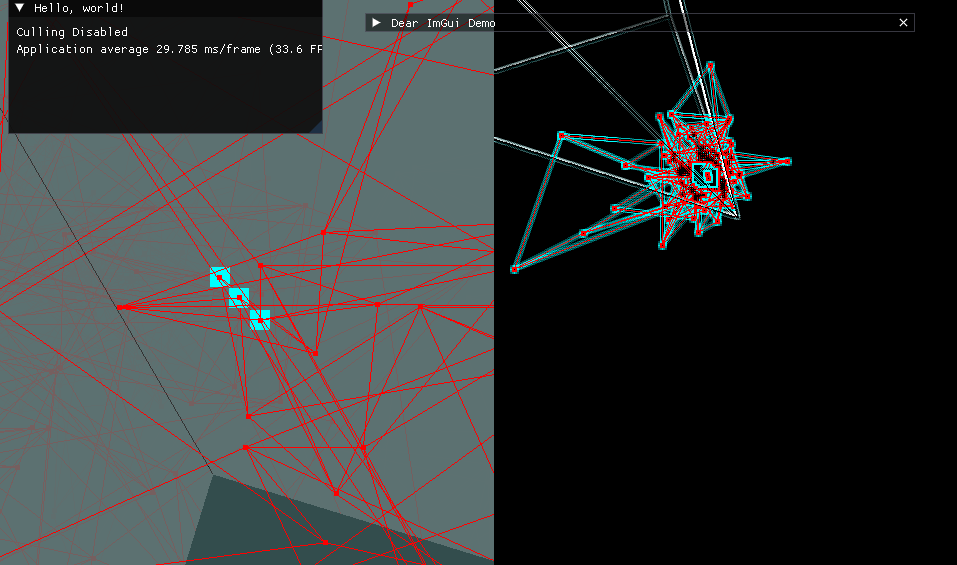
\includegraphics[width=0.45\textwidth,keepaspectratio]{chaos1.PNG}
                \caption{Chaos.}
                \label{"fig:chaos"}
        \end{figure}

        \subsection{Degeneracies}
        It is known that the DEP/S algorithm is prone to some degeneracies, such as when an edge collapses or when the altitude collapses \cite{Tamstorf2013discrete}. This may manifest int the calculation as a division by zero error during the solve, an infinite loop (the error never reaches the desired tolerance), or the cloth visually becomes a cloud of points (see figure \ref{"fig:chaos"}). This is more apparent in simulations with more DOFs as there is more room for numerical instability to occur. Thus, it may be prudent to check for ways to alleviate and prevent these degeneracies from occurring.

        \subsection{Scope Changes}
        In my initial proposal, I mentioned the potential to allow computation to run on the GPU, specifically the solver\cite{bolz2003sparse}. However I amd going to cut this feature for the project for 2 main reasons: 1) OpenGL does not have a built in matrix solver, only capable of calculating inverses and 2) OpenGL does not support matrices with dimensions greater than 4x4, so basic matrix operations like matrix multiplication, matrix addition, and matrix solve would need to be implemented by hand. This is out of scope for this project and better left as an exercise at a later time. Additionally, lighting and other aesthetics are also out of scope for this project due to the limitations of my current renderer design and the time constraints of the project. It is currently more important to focus more on the optimization of the simulation and addressing the degeneracies that may occur.



\section{Conclusion}

        In this midterm report, I discussed the progress I made in the cloth simulation project, the problems I encountered, and the future plans I have for the project. I have a working implementation of the cloth simulation in C++ and have identified the areas for optimization and the mitigations for the degeneracies that may occur in the simulation. Hopefully, these issues will be addressed in the next week before the final presentation.



\addtolength{\textheight}{-12cm}   % This command serves to balance the column lengths
                                  % on the last page of the document manually. It shortens
                                  % the textheight of the last page by a suitable amount.
                                  % This command does not take effect until the next page
                                  % so it should come on the page before the last. Make
                                  % sure that you do not shorten the textheight too much.

%%%%%%%%%%%%%%%%%%%%%%%%%%%%%%%%%%%%%%%%%%%%%%%%%%%%%%%%%%%%%%%%%%%%%%%%%%%%%%%%



%%%%%%%%%%%%%%%%%%%%%%%%%%%%%%%%%%%%%%%%%%%%%%%%%%%%%%%%%%%%%%%%%%%%%%%%%%%%%%%%

\bibliographystyle{ieeetr} % We choose the "plain" reference style
\bibliography{refs} % Entries are in the refs.bib file

\end{document}
